\documentclass[11pt,reqno]{amsart}
\usepackage[T1]{fontenc}
\usepackage[utf8]{inputenc}
\usepackage{lmodern,microtype,amsmath,amssymb,amsthm,mathtools}
\usepackage{graphicx,booktabs,longtable,array,xcolor,placeins}
\usepackage{tikz}
\usetikzlibrary{arrows.meta,positioning,fit,backgrounds}
\usepackage[colorlinks=true,linkcolor=blue!45!black,citecolor=blue!45!black,urlcolor=blue!45!black]{hyperref}
\hypersetup{pdftitle={Sensor Coverage under Structured Failures},pdfauthor={Deep Bhattacharjee; Ushashi Bhattacharya; Sanjeevan Singha Roy}}
\usepackage[capitalise,noabbrev]{cleveref}
\setlength{\textwidth}{6.1in}
\setlength{\oddsidemargin}{.2in}
\setlength{\evensidemargin}{.2in}
\setlength{\textheight}{8.65in}
\setlength{\topmargin}{0in}
\setcounter{tocdepth}{1}
\renewcommand{\topfraction}{.9}
\renewcommand{\textfraction}{.08}
\renewcommand{\floatpagefraction}{.5}
\newtheorem{theorem}{Theorem}[section]
\newtheorem{proposition}[theorem]{Proposition}
\newtheorem{lemma}[theorem]{Lemma}
\newtheorem{corollary}[theorem]{Corollary}
\theoremstyle{definition}
\newtheorem{definition}[theorem]{Definition}
\newtheorem{example}[theorem]{Example}
\newtheorem{algorithm}[theorem]{Algorithm}
\theoremstyle{remark}
\newtheorem{remark}[theorem]{Remark}
\newcommand{\R}{\mathbb R}
\newcommand{\F}{\mathcal F}
\newcommand{\M}{\mathcal M}
\newcommand{\W}{\mathcal W}
\newcommand{\cC}{\mathcal C}
\newcommand{\cP}{\mathcal P}
\newcommand{\FF}{\mathbb F_2}
\newcommand{\abs}[1]{\left|#1\right|}
\DeclareMathOperator{\rank}{rank}
\DeclareMathOperator{\sd}{sd}
\DeclareMathOperator{\conv}{conv}
\DeclareMathOperator{\diam}{diam}
\DeclareMathOperator{\im}{im}
\DeclareMathOperator{\Max}{Max}
\DeclareMathOperator{\Min}{Min}
\title[Sensor coverage under structured failures]{Sensor Coverage under Structured Failures}
\author{Deep Bhattacharjee}
\address{Electro-Gravitational Space Propulsion Laboratory (EGSPL), Bhubaneswar, Odisha, India}
\email{itsdeep@live.com}
\urladdr{https://orcid.org/0000-0003-0466-750X}
\author{Ushashi Bhattacharya}
\address{Dortmund, Germany; National Taiwan University, Taipei, Taiwan}
\author{Sanjeevan Singha Roy}
\address{Formerly, Birla Institute of Technology (BIT) Mesra, India}
\email{sanjeevan9905@gmail.com}
\urladdr{https://orcid.org/0000-0002-6148-1421}
\date{Version 3.0.1, October 28, 2026}
\subjclass[2020]{Primary 55U10; Secondary 55N31, 68U05, 90B18}
\keywords{sensor coverage, structured failures, Dowker duality, multicover, exact geometric predicates, target certificates}
\thanks{This manuscript is a substantially revised version of \emph{Iterated Nerve Complexes for $k$-Fold Sensor Coverage}, Preprints.org, DOI: 10.20944/preprints202606.1351.v2. The title, scope, proofs and computations have been revised.}
\begin{document}
\begin{abstract}
We study the part of a sensor field that remains covered after every failure in a prescribed downward-closed family. The model includes independent contact failures, weighted failure budgets and losses of entire fault domains. For a convex sensor cover with nerve $N$, we express the surviving region by a complex on the maximal faces of $N$: a collection of maximal faces is a simplex exactly when its common contact set cannot fail. This is a coverage formulation of classical nerve and Dowker duality, for which we give explicit comparison maps and prove naturality under increasing failure families. For $n$ closed planar disks, all maximal nerve faces are witnessed by at most $n^2$ circle points. Exact rational sign tests consequently construct the full two-skeleton of the dual model without enumerating the original nerve or the coalition shadow. A separate Lipschitz margin theorem gives continuous coverage certificates for prescribed triangulated targets under the same failure rules. Recomputing five supplied fields completes the previously unfinished dense example: its two-fold covered region has Betti numbers $(5,6)$, calculated from a dual complex with $130$ vertices and independently checked boundary rank. The implementation, inputs, exact arithmetic conventions and verification records are supplied.
\end{abstract}
\maketitle
\tableofcontents
\section{Introduction}
\label{sec:intro}
Redundant coverage is often specified as an overlap count: every point should lie in at least $k$ footprints. That specification is adequate when any $k-1$ individual contacts may fail. It can be inadequate when several contacts share a power source, communication link or acquisition channel. Two contacts in the same failed group provide no surviving measurement, even though their footprints give two-fold coverage. The appropriate mathematical input is therefore a family of allowed failures, together with the geometric footprints.

The ordinary nerve records which collections of footprints have a common point. Classical nerve theory identifies the topology of their union, while multicover constructions recover the regions of higher overlap. Our starting point is the earlier two-author manuscript~\cite{original}, whose $k$-shadow is the nerve of the family of $k$-wise footprint intersections. The underlying multicover equivalence is an application of the nerve theorem. It is part of an established literature, including Sheehy's multicover nerve~\cite{sheehy}, the multicover bifiltration of Corbet, Kerber, Lesnick and Osang~\cite{corbet}, and Alonso's sparse approximation~\cite{alonso}. We do not claim to introduce the first nerve model of multiple coverage or a new general Dowker theorem.

The present revision addresses a different practical question. Can one evaluate coverage for a general monotone failure rule without first constructing every coalition vertex and every high-dimensional face of the original nerve? We use the maximal faces of the nerve as vertices of a dual complex. Their intersection supplies the contact set on which the failure rule is evaluated. The construction is a direct instance of Dowker duality~\cite{dowker,chowdhury}; its use here makes the failure semantics explicit and permits a geometry-first implementation.

\subsection{Statements and computational outcome}
Write $D_1,\ldots,D_n$ for compact convex sensor footprints and let $\F\subseteq 2^{[n]}$ be a downward-closed family containing the empty set. A member of $\F$ is a contact set that is allowed to fail. The region of guaranteed survival is
\begin{equation}\label{eq:survival-intro}
R_{\F}=\bigcap_{F\in\F}\ \bigcup_{i\notin F}D_i.
\end{equation}
Let $N$ be the nerve of the footprints and $\M=\Max N$ its maximal faces. Define the nonempty simplices of a complex by
\begin{equation}\label{eq:dual-intro}
\cC_{\F}(N)=\left\{A\subseteq\M:A\ne\varnothing,\quad \bigcap_{M\in A}M\notin\F\right\}.
\end{equation}
Singletons that do not satisfy the displayed rule are absent; thus not every member of $\M$ is necessarily a vertex.

\Cref{thm:duality} proves $\abs{\cC_{\F}(N)}\simeq R_{\F}$. Its combinatorial proof gives explicit order maps rather than relying on a count of faces or a raster image. \Cref{thm:natural} treats inclusions of failure families at fixed geometry. \Cref{thm:witness} proves that all maximal faces for planar disks occur among the contact labels of at most $n^2$ circle points. \Cref{thm:algorithm} turns this observation into an exact finite algorithm for $H_0$ and $H_1$. \Cref{thm:target} supplies a sufficient continuous target certificate, separately from any homology computation.

The dense Field~E of~\cite{original} contains $95$ equal-radius disks. The previous two-fold shadow computation stopped before its triangle boundary rank was obtained. The dual calculation gives
\begin{equation}\label{eq:E-result}
\begin{split}
(V,E,T)&=(130,4214,94985),\\
\rank\partial_2&=4083,\qquad (b_0,b_1)=(5,6).
\end{split}
\end{equation}
The full two-skeleton is included in this count. There is no cutoff on clique size, no omitted triangle class and no substitution of pairwise overlap for common intersection.

\subsection{What is corrected from version 2}
Two distinctions matter for the interpretation of the earlier computations. First, the reported number $836\,991$ in the dense example counts \emph{edges} of the two-fold shadow, not its vertices. Its vertices are the $1810$ edges of the ordinary nerve. We recount these quantities in \cref{sec:experiments}. Second, vanishing first homology does not establish that a specified target lies inside the covered region. A contractible disk far from a target has $b_1=0$ while leaving that target entirely uncovered. The target test developed below is a separate sufficient criterion.

These corrections do not invalidate the elementary nerve equivalence for the secondary cover. They change the size interpretation and the conclusion that can be drawn from a Betti number. We record both corrections explicitly so that the present version can be read against the archived v2.

\subsection{Relation to prior work}
The homological study of sensor coverage includes the work of Ghrist and Muhammad~\cite{ghrist}, and the persistent and controlled-boundary criteria of de Silva and Ghrist~\cite{desilva,controlled}. Those criteria include hypotheses concerning boundaries and relative homology; they are not interchangeable with the assertion $b_1=0$. The finite closed-convex nerve theorem and its functorial forms are treated systematically in~\cite{bauer}. Dowker's relation complexes and their functorial extension~\cite{dowker,chowdhury} explain the duality used in this paper.

Our companion ECoG archive~\cite{ecog} distinguishes exact intersection predicates, target mesh certification and numerical illustrations. We retain that distinction and extend the margin argument to arbitrary monotone failure rules. Earlier work of the authors on circuit topoi~\cite{topoi}, topological deformation~\cite{suspension}, and stability of linked spaces~\cite{linkage} provides broader context for local-to-global network questions. These latter references are contextual; none of their claims is a premise of a proof here. The geometry, combinatorial maps and chain calculations required below are specified directly.

\subsection{Conventions}
All abstract complexes are finite. Empty faces are understood, but face posets contain only nonempty faces. The realization of a complex with no vertices is empty, and its ordinary $H_0$ is zero. Unless stated otherwise, homology is ordinary homology over $\FF$. The topological theorems also hold with any fixed field of coefficients. Footprints in the general topological statements are compact convex subsets of a Euclidean space. Exact enumeration and the numerical experiments concern \emph{closed} disks in $\R^2$.

The distinction between open and closed footprints is material at tangency. In the supplied fields the independent pair and triple check detects no exact tangency, but the implementation also tests tangent and coincident examples. All claims of numerical exactness refer to the finite binary64 input numbers interpreted as rational numbers; they are not claims of exact knowledge of physical sensor positions.

\begin{figure}[tb]
\centering
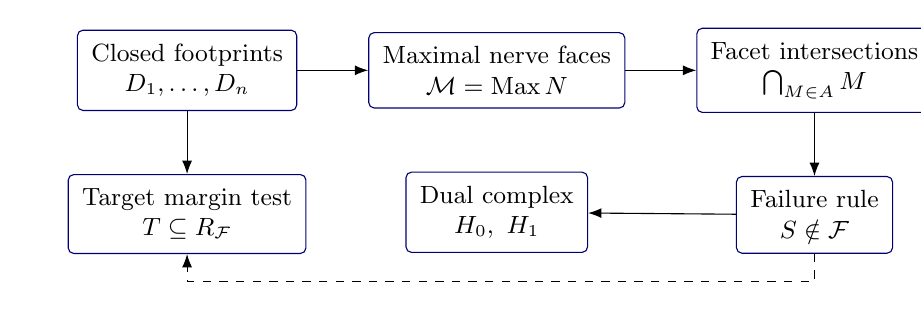
\begin{tikzpicture}[node distance=8mm and 9mm,box/.style={draw=blue!45!black,rounded corners=2pt,align=center,inner sep=5pt,font=\small},>=Latex]
\node[box] (geo) {Closed footprints\\$D_1,\ldots,D_n$};
\node[box,right=of geo] (fac) {Maximal nerve faces\\$\M=\Max N$};
\node[box,right=of fac] (dual) {Facet intersections\\$\bigcap_{M\in A}M$};
\node[box,below=of dual] (test) {Failure rule\\$S\notin\F$};
\node[box,below=of fac] (hom) {Dual complex\\$H_0,\ H_1$};
\node[box,below=of geo] (target) {Target margin test\\$T\subseteq R_{\F}$};
\draw[->] (geo)--(fac);\draw[->] (fac)--(dual);\draw[->] (dual)--(test);
\draw[->] (test)--(hom);\draw[->] (geo)--(target);
\draw[->,dashed] (test.south) -- ++(0,-.35) -| (target.south);
\end{tikzpicture}
\caption{Two outputs from one failure rule. The dual complex determines topology. A margin certificate establishes coverage of a prescribed target. Neither output is silently substituted for the other.}
\label{fig:workflow}
\end{figure}

\section{Failure families and surviving regions}
\label{sec:failures}
\begin{definition}
A \emph{failure family} is a downward-closed set $\F\subseteq2^{[n]}$ with $\varnothing\in\F$. Its complement $\W=2^{[n]}\setminus\F$ is the family of \emph{winning contact sets}. Thus $S\in\W$ and $S\subseteq S'$ imply $S'\in\W$. The active contact set at $x$ is
\[
S(x)=\{i\in[n]:x\in D_i\}.
\]
\end{definition}
The word ``winning'' refers solely to survival of the prescribed failure model. It does not encode a probability, sensor independence or a clinical performance measure.

\begin{proposition}[Pointwise failure reduction]\label{prop:pointwise}
For every $x$ the following conditions are equivalent:
\begin{enumerate}
\item $x$ remains covered after every failure $F\in\F$;
\item $S(x)\notin\F$;
\item some $\sigma\subseteq S(x)$ is a minimal member of $\W$.
\end{enumerate}
Consequently, with $D_\sigma=\bigcap_{i\in\sigma}D_i$ and $\cP_{\F}=\{\sigma\in N:\sigma\notin\F\}$,
\begin{equation}\label{eq:region-unions}
R_{\F}=\bigcup_{\sigma\in\cP_{\F}}D_\sigma
=\bigcup_{\sigma\in\Min\W}D_\sigma,
\end{equation}
where empty geometric intersections contribute nothing.
\end{proposition}
\begin{proof}
Failure of coverage at $x$ after deleting $F$ means precisely that every active contact is deleted: $S(x)\subseteq F$. If $F\in\F$, downward closure then gives $S(x)\in\F$. Conversely, if $S(x)\in\F$, the allowed choice $F=S(x)$ deletes every active contact. This proves the equivalence of the first two statements. In a finite upward-closed family every member contains a minimal member, and any set containing a winning set is winning. This proves the third equivalence and both union identities.
\end{proof}

\begin{example}[Independent failures]
For an integer $q\ge0$, let $\F_q=\{F:\abs F\le q\}$. A set wins exactly when it contains at least $q+1$ contacts. Thus $R_{\F_q}$ is the ordinary $(q+1)$-fold covered region. For $q\ge n$ it is empty.
\end{example}

\begin{example}[Weighted failure budgets]\label{ex:weighted}
Give contact $i$ a nonnegative integer failure cost $c_i$ and fix an integer budget $B\ge0$. Set
\[
\F_{c,B}=\left\{F:\sum_{i\in F}c_i\le B\right\}.
\]
Then
\begin{equation}\label{eq:weighted-rule}
S\in\W\quad\Longleftrightarrow\quad\sum_{i\in S}c_i>B.
\end{equation}
This is an adversarial deletion-cost model. It is not a statement that measurements have additive quality or that physical reliability is proportional to $c_i$. Zero-cost contacts can be deleted freely; the formula still applies. Nonintegral nonnegative costs also define a mathematical failure family, but the supplied budget implementation deliberately accepts only integers.
\end{example}

\begin{example}[Correlated fault domains]\label{ex:domains}
Partition contacts into labeled domains $G_1,\ldots,G_s$ and allow the loss of any $q$ complete domains. Its downward closure is
\[
\F_{G,q}=\{F:F\subseteq\textstyle\bigcup_{j\in J}G_j\text{ for some }\abs J\le q\}.
\]
If $d(S)=\{j:S\cap G_j\ne\varnothing\}$, the winning rule is
\begin{equation}\label{eq:domain-rule}
S\in\W\quad\Longleftrightarrow\quad\abs{d(S)}>q.
\end{equation}
Indeed, at most $q$ domains contain $S$ exactly when all its active domains can be deleted. The downward closure includes partial deletions, but its universal survival region equals that of the allowed complete-domain losses: any partial deletion is contained in one of those losses.
\end{example}

\begin{example}[Two-fold coverage can fail a one-domain test]
Take two identical disks and assign both contacts to one domain. Their common disk is two-fold covered. Deleting that domain leaves no coverage. If instead the two contacts belong to different domains, the same geometry survives every loss of one domain. Ordinary overlap counts and the ordinary nerve without domain labels cannot distinguish these two reliability requirements.
\end{example}

\begin{proposition}[Combining requirements]\label{prop:combining}
If $\F_1,\F_2$ are failure families, then
\[
R_{\F_1\cup\F_2}=R_{\F_1}\cap R_{\F_2},\qquad
R_{\F_1\cap\F_2}=R_{\F_1}\cup R_{\F_2}.
\]
Both union and intersection on the left are downward closed.
\end{proposition}
\begin{proof}
At each point, the first equality says that $S(x)$ belongs to neither failure family. The second says that it does not belong to both. Apply De Morgan's laws to \cref{prop:pointwise}.
\end{proof}

For a simultaneous requirement of a budget bound and a domain-loss bound one must specify whether the adversary may use either rule separately, both at once, or a composed deletion. These are different failure families. The framework accepts each, but it does not identify them without a stated model.

\begin{example}[Independence systems]
An independence system on $[n]$ is, by definition, downward closed. Taking it as $\F$ makes its dependent sets the winning coalitions. For a matroid, the minimal winning coalitions are its circuits. This observation is a translation of definitions; no matroid representation hypothesis is needed for the dual construction. The number of minimal winning coalitions can nevertheless be large, which is a reason to evaluate a winning predicate on facet intersections instead of listing all such coalitions.
\end{example}

\begin{lemma}[Monotonicity]\label{lem:monotonicity}
If $D_i\subseteq D_i'$ for every label $i$, then $R_{\F}(D)\subseteq R_{\F}(D')$. If $\F_1\subseteq\F_2$, then $R_{\F_2}(D)\subseteq R_{\F_1}(D)$.
\end{lemma}
\begin{proof}
In the first case $S_D(x)\subseteq S_{D'}(x)$ and winning is upward closed. In the second case $S(x)\notin\F_2$ implies $S(x)\notin\F_1$.
\end{proof}

\section{The facet-intersection model}
\label{sec:duality}
Let $N$ be the nerve of a finite family of nonempty compact convex sets. Every face lies in a maximal face. Empty footprints can be removed beforehand without changing any pointwise active set on the remaining labels. Keep the failure rule restricted to those labels.

\begin{definition}
The \emph{winning-face complex} $\Gamma_{\F}(N)$ has one vertex for each $\sigma\in\cP_{\F}$. A nonempty collection $A$ of its vertices is a simplex if
\begin{equation}\label{eq:Gamma}
\bigcup_{\sigma\in A}\sigma\in N.
\end{equation}
The \emph{facet-intersection complex} $\cC_{\F}(N)$ is given by \cref{eq:dual-intro}.
\end{definition}
Upward closure of winning sets implies that \cref{eq:dual-intro} is closed under taking nonempty subsets of $A$: removing a maximal face makes the intersection larger. Thus it does define an abstract simplicial complex. In contrast, enlarging a contact set in $N$ need not preserve being a face, so the directions of the union and intersection tests must not be reversed.

\begin{theorem}[Coverage duality]\label{thm:duality}
For compact convex footprints and any failure family,
\begin{equation}\label{eq:homotopy-chain}
R_{\F}\simeq\abs{\Gamma_{\F}(N)}\simeq\abs{\cC_{\F}(N)}.
\end{equation}
The combinatorial equivalence is an instance of Dowker duality for the containment relation between winning faces and maximal nerve faces. It does not require a bound on the sizes of those faces.
\end{theorem}
\begin{proof}
By \cref{prop:pointwise}, the sets $D_\sigma$, indexed by $\sigma\in\cP_{\F}$, cover $R_{\F}$. A finite intersection of these sets is
\[
\bigcap_{\sigma\in A}D_\sigma=D_{\bigcup_{\sigma\in A}\sigma}.
\]
It is nonempty exactly when \cref{eq:Gamma} holds, and when nonempty it is compact and convex. The finite closed-convex nerve theorem therefore identifies its nerve $\Gamma_{\F}(N)$ with $R_{\F}$ up to homotopy. The closed-convex hypothesis is used here; an arbitrary cover by closed contractible sets would not justify the same argument~\cite{bauer}.

For completeness, we prove the combinatorial equivalence by explicit maps. Let $Q_\Gamma$ and $Q_C$ be the nonempty face posets of $\Gamma_{\F}(N)$ and $\cC_{\F}(N)$. Set
\begin{align}
f(A)&=\left\{M\in\M:\bigcup_{\sigma\in A}\sigma\subseteq M\right\},\label{eq:f-map}\\
g(B)&=\left\{\sigma\in\cP_{\F}:\sigma\subseteq\bigcap_{M\in B}M\right\}.\label{eq:g-map}
\end{align}
For a face $A$, its union is in $N$, so $f(A)$ is nonempty. The intersection of all members of $f(A)$ contains that union, which contains a winning face. Hence $f(A)$ is a face of $\cC_{\F}$. For a face $B$, its intersection $I_B$ is a winning face of $N$. In particular, $I_B\in g(B)$, and the union of all members of $g(B)$ is exactly $I_B$. Thus $g(B)$ is a nonempty face of $\Gamma_{\F}$.

Both maps reverse inclusion. Their composites preserve inclusion and satisfy
\begin{equation}\label{eq:closure-inequalities}
A\subseteq g f(A),\qquad B\subseteq f g(B).
\end{equation}
For the first inclusion, each $\sigma\in A$ lies in every maximal face containing the union of $A$. For the second, $\bigcup g(B)=I_B$ lies in every $M\in B$.

An order-preserving map pointwise above the identity induces a map homotopic to the identity on the order complex; a proof by prisms is given in \cref{app:posets}. An order-reversing map also induces a simplicial map on order complexes, by reversing the order of each image chain. Applying this observation to \cref{eq:closure-inequalities}, the realizations of $f$ and $g$ are mutually inverse up to homotopy. The order complexes are the barycentric subdivisions of $\Gamma_{\F}$ and $\cC_{\F}$, whose realizations are homeomorphic to those of the original complexes.

If there is no winning nerve face, all three spaces are empty by definition and the assertion is immediate.
\end{proof}

\begin{corollary}[Minimal-coalition shadow]\label{cor:minimal}
Let $\Lambda_{\F}=\Min\W\cap N$. Form a complex on $\Lambda_{\F}$ by declaring $A$ a face when $\bigcup_{\sigma\in A}\sigma\in N$. Its realization is homotopy equivalent to $R_{\F}$ and to $\abs{\cC_{\F}(N)}$. For $\F=\F_{k-1}$ this is exactly the $k$-shadow $\Delta_k(N)$.
\end{corollary}
\begin{proof}
The subfamily $(D_\sigma)_{\sigma\in\Lambda_{\F}}$ is still a finite convex cover of $R_{\F}$ by \cref{eq:region-unions}. Its nerve is the stated union complex. Apply the same closed-convex nerve theorem and \cref{thm:duality}.
\end{proof}

Using every winning face in $\Gamma_{\F}$ is convenient for naturality but unnecessary in the implementation. Using only minimal winners is often still expensive. The dual complex evaluates the predicate only on intersections of maximal nerve faces and does not list either collection of coalitions.

\begin{theorem}[Increasing failure families]\label{thm:natural}
Fix the footprints, their nerve $N$ and its full set of maximal faces $\M$. If $\F_1\subseteq\F_2$, there are inclusions
\[
\Gamma_{\F_2}\subseteq\Gamma_{\F_1},\qquad
\cC_{\F_2}\subseteq\cC_{\F_1},\qquad
R_{\F_2}\subseteq R_{\F_1}.
\]
For every homological degree and fixed coefficient field the isomorphisms in \cref{thm:duality} can be taken natural for these inclusions. Therefore a nested sequence of failure families gives isomorphic homology persistence modules in the geometric and dual models.
\end{theorem}
\begin{proof}
A face winning against $\F_2$ wins against $\F_1$, proving the first two inclusions directly from their defining tests. The region inclusion is \cref{lem:monotonicity}. On nonempty face posets the map $f$ in \cref{eq:f-map} is independent of the failure family: it lists all maximal faces containing a given union. Hence its square with the two inclusion maps commutes exactly. Since $f$ is an objectwise homotopy equivalence, it induces a natural homology isomorphism.

The convex cover for $\F_2$ is a subfamily of the one for $\F_1$, with the same geometric set attached to each surviving index. The functorial closed-convex nerve theorem supplies natural homology isomorphisms for this inclusion. In the disk setting, compatible semialgebraic triangulations and the double-chain comparison in \cref{app:nerve} give an additional chain-level explanation. Composing the two comparisons proves the assertion.
\end{proof}

\begin{remark}[Changing geometry]
Maximal nerve faces can change when radii or positions change. The literal vertex sets of the corresponding facet-intersection complexes then need not be nested. \Cref{thm:natural} fixes the geometry; it does not assert a raw simplicial inclusion for moving radii. Geometric perturbation inclusions are proved in \cref{sec:certificates}, and standard multicover bifiltrations already address simultaneous radius and multiplicity parameters~\cite{corbet,alonso}.
\end{remark}

\begin{proposition}[Two-skeleton sufficiency]\label{prop:two-skeleton}
For any finite complex $K$, its full two-skeleton determines $H_0(K;\FF)$ and $H_1(K;\FF)$. If its graph has $V$ vertices, $E$ edges and $c$ components, then
\begin{equation}\label{eq:betti-formula}
b_0=c,\qquad b_1=E-V+c-\rank\partial_2.
\end{equation}
\end{proposition}
\begin{proof}
The chain groups and boundary maps relevant to degrees zero and one are
\[
C_2(K;\FF)\xrightarrow{\partial_2}C_1(K;\FF)\xrightarrow{\partial_1}C_0(K;\FF).
\]
Higher-dimensional simplices do not change these maps. In the graph of $K$, the incidence matrix has rank $V-c$: a spanning tree gives rank $v-1$ on a connected component with $v$ vertices, and every additional edge has boundary equal to the sum of boundaries along its tree path. Thus $\dim\ker\partial_1=E-V+c$. Quotient by $\im\partial_2$ to obtain \cref{eq:betti-formula}.
\end{proof}

\begin{example}[The dual complex need not be a flag complex]
Take maximal nerve faces $M_1=\{1,2\}$, $M_2=\{2,3\}$ and $M_3=\{1,3\}$, with the rule that one contact suffices. Every pair of maximal faces intersects in a winning singleton, but all three have empty intersection. The dual complex has three edges and no triangle. Filling its graph clique would erase its first homology. The implementation checks the three-fold facet intersection for every candidate triangle.
\end{example}

\section{Exact geometry without nerve-face enumeration}
\label{sec:geometry}
The duality theorem is useful only if the maximal nerve faces can be obtained reliably. For disks, a finite arrangement construction avoids listing every intersecting subfamily. In this section
\[
D_i=\{x\in\R^2:\|x-c_i\|\le r_i\},\qquad r_i\ge0,
\]
and coincident disks keep their distinct contact labels.

\begin{definition}
The \emph{witness list} consists of the leftmost point $\ell_i=(c_{i,x}-r_i,c_{i,y})$ of each disk and all intersections of the boundaries of pairs of disks whose supporting circles are distinct. A zero-radius disk contributes its center through $\ell_i$. A coincident pair contributes no additional points. The label of a witness $x$ is $L(x)=\{i:x\in D_i\}$.
\end{definition}

\begin{theorem}[Quadratic witness bound]\label{thm:witness}
Every maximal face of the nerve is the label of a point on the witness list. Hence the inclusion-maximal nonempty witness labels are exactly $\Max N$, and
\begin{equation}\label{eq:witness-count}
\abs{\Max N}\le n+2\binom n2=n^2.
\end{equation}
The assertion allows unequal radii, tangency, zero radii and coincident disks.
\end{theorem}
\begin{proof}
Every witness label is a nerve face, because the witness itself lies in all its labeled disks. Let $\sigma$ be a maximal nerve face and set $K=\bigcap_{i\in\sigma}D_i$. This is nonempty and compact. Choose a point $x\in K$ with minimal first coordinate.

If $\sigma$ contains a zero-radius disk, then $K$ consists of its center, which is a listed witness. Suppose all its disks have positive radius. At least one constraint is active at $x$: if all were strict, a small open neighborhood of $x$ would lie in $K$, contradicting minimality. If two active constraints have distinct supporting circles, $x$ is one of their boundary intersections and is listed.

The remaining case has only one distinct active supporting circle, possibly repeated with several labels. Every other disk of $\sigma$ contains a neighborhood of $x$. In a sufficiently small neighborhood the only effective constraint is therefore the closed disk bounded by that active circle. Unless $x$ is its leftmost point, there are points of that disk arbitrarily close to $x$ with smaller first coordinate. They still satisfy every locally slack constraint, a contradiction. Thus $x$ is the leftmost point of an active disk and is listed.

In all cases $\sigma\subseteq L(x)$. The label is a nerve face and $\sigma$ is maximal, so equality follows. Taking maximal labels removes only proper subfaces and duplicates. Each noncoincident pair of circles has at most two intersection points, which proves \cref{eq:witness-count}.
\end{proof}

\begin{remark}
The extremal-point argument is an elementary disk-arrangement method. The bound concerns the number of maximal nerve faces, not the number of all nerve faces or all simplices of the dual complex. A single maximal face on $n$ labels contains $2^n-1$ nonempty nerve faces. Likewise $n^2$ dual vertices alone do not give a quadratic bound on all dual simplices.
\end{remark}

\subsection{Circle intersections in a quadratic extension}
The witness labels can be determined without evaluating square roots approximately. Suppose $c_i\ne c_j$ and put
\begin{align}
d&=c_j-c_i,\qquad s=d\cdot d>0,\nonumber\\
\alpha&=\frac{s+r_i^2-r_j^2}{2s},\qquad
h=\frac{r_i^2}{s}-\alpha^2,\label{eq:circle-parameters}\\
B&=c_i+\alpha d,\qquad P=(-d_y,d_x).\nonumber
\end{align}
If $h<0$, the boundaries do not meet. If $h=0$, they meet at $B$. If $h>0$, their intersections are
\begin{equation}\label{eq:circle-points}
x_{\pm}=B\pm\sqrt h\,P.
\end{equation}
Indeed, subtracting the two circle equations gives the line $(x-c_i)\cdot d=\alpha s$. Substituting $x=B+tP$ in the first equation gives $t^2=h$. This also covers internal and external tangency.

For a third disk, write $z=B-c_k$. Membership of $x_\pm$ is the inequality
\begin{equation}\label{eq:quadratic-membership}
A+C\sqrt h\le0,
\quad A=z\cdot z+h(P\cdot P)-r_k^2,
\quad C=\pm2z\cdot P.
\end{equation}
When input numbers are rational, $A,C,h$ are rational. No coordinates of a square-root point need be rounded.

\begin{lemma}[Exact radical sign]\label{lem:sign}
Let $A,C,h\in\mathbb Q$ with $h\ge0$. The truth of $A+C\sqrt h\le0$ is determined by rational comparisons as follows:
\begin{enumerate}
\item if $h=0$ or $C=0$, test $A\le0$;
\item if $A=0$ and $h>0$, test $C\le0$;
\item if $A<0$ and $C<0$, the inequality holds; if $A>0$ and $C>0$, it fails;
\item if $A>0$ and $C<0$, test $A^2\le C^2h$;
\item if $A<0$ and $C>0$, test $C^2h\le A^2$.
\end{enumerate}
\end{lemma}
\begin{proof}
The first three cases follow from signs. In the fourth case the desired inequality is $A\le(-C)\sqrt h$, with both sides nonnegative, so squaring preserves its direction and equivalence. In the fifth case it is $C\sqrt h\le -A$, again with nonnegative sides. These cases exhaust all possibilities. Equality is retained because the disks are closed.
\end{proof}

\subsection{Enumeration and chain construction}
\begin{algorithm}[Exact facet computation]\label{alg:facets}
\leavevmode
\begin{enumerate}
\item Interpret the finite coordinates and radii as rationals; reject negative radii or nonfinite input.
\item Label the $n$ leftmost points by squared-distance comparisons.
\item For each pair of distinct centers, compute \cref{eq:circle-parameters}. If $h\ge0$, label its one or two boundary intersections using \cref{lem:sign}. Pairs with equal centers require no boundary computation.
\item Delete empty labels and duplicates. Sort the remaining masks by decreasing cardinality, and retain a mask exactly when it is not contained in a previously retained mask.
\end{enumerate}
The output is $\Max N$ by \cref{thm:witness}.
\end{algorithm}

With $m=\abs\M$ and a winning predicate $w$, the full dual two-skeleton is constructed as follows. Retain $M\in\M$ as a vertex if $w(M)$ is true. An edge $\{M_i,M_j\}$ is retained if $w(M_i\cap M_j)$ is true. A candidate triangle is retained if all three edges exist and $w(M_i\cap M_j\cap M_k)$ is true. The edge checks are redundant mathematically for an upward-closed rule, but they avoid unnecessary work and ensure a consistent boundary indexing.

Each triangle gives a boundary column with three nonzero edge entries over $\FF$. Gaussian elimination determines its rank, while a union--find structure computes the graph components. \Cref{eq:betti-formula} then gives both Betti numbers.

\begin{theorem}[Finite exact low-degree computation]\label{thm:algorithm}
For $n$ closed planar disks with rational input data, and an exactly evaluable monotone winning predicate, \cref{alg:facets} and the complete dual two-skeleton compute $H_0$ and $H_1$ of the surviving region exactly over $\FF$. Witness labeling uses $O(n^3)$ rational sign tests. A naive maximal-label filter uses $O(n^4)$ mask-containment tests. The dual two-skeleton uses at most $n^2$ vertices, $\binom{n^2}{2}$ edge predicates and $\binom{n^2}{3}$ triangle predicates.
\end{theorem}
\begin{proof}
There are at most $n^2$ witnesses and $n$ membership tests per witness. A quadratic comparison of at most $n^2$ labels bounds the naive filtering step. Correctness of those steps follows from \cref{thm:witness,lem:sign}. The simplex count follows from $m\le n^2$, and every simplex through dimension two is included by its defining predicate. \Cref{thm:duality,prop:two-skeleton} identify the resulting homology with that of the surviving region.
\end{proof}

This is an arithmetic-operation and oracle-query bound. It is not a unit-time bit-complexity bound: rational numerator sizes, arbitrary-precision mask operations, predicate costs and elimination all matter. The worst-case number of dual triangles is $O(n^6)$, and the full dual complex may have exponentially many simplices. For $H_j$ with fixed $j$, its full $(j+1)$-skeleton suffices, giving at most $O(n^{2j+4})$ simplex tests by the same argument. These bounds are deliberately separate from the much more refined multicover bifiltration algorithms of~\cite{corbet,alonso}.

\subsection{Equal-radius verification by a different geometric formula}
The data fields use a common radius $r$. Their geometry can therefore be checked independently by minimum enclosing circles of center triples. If $a,b,c$ are three centers, let
\[
u=\|a-b\|^2,\quad v=\|a-c\|^2,\quad w=\|b-c\|^2,
\quad J=(b-a)_x(c-a)_y-(b-a)_y(c-a)_x.
\]
The squared minimum enclosing radius is
\begin{equation}\label{eq:mec}
\rho^2(a,b,c)=
\begin{cases}
\max(u,v,w)/4,&2\max(u,v,w)\ge u+v+w,\\[2pt]
uvw/(4J^2),&2\max(u,v,w)<u+v+w.
\end{cases}
\end{equation}
The first case includes right, obtuse, collinear and coincident configurations. The second is the circumradius formula for an acute triangle; its denominator is nonzero. Two equal-radius disks meet if their center distance squared is at most $4r^2$, and three meet if and only if $\rho^2\le r^2$. Planar Helly's theorem extends the triple criterion to every larger subfamily.

The verification script uses \cref{eq:mec}, not the circle-witness formulas. It compares every pair and triple with the facet face oracle, checks that every returned facet is a face and that every one-contact extension fails, and independently reduces the two-fold boundary matrix using set columns and the opposite pivot order. Completeness of the witness list is supplied by \cref{thm:witness}; checking triples alone would not, for an arbitrary list of purported facets, prove that completeness.

\section{Continuous target certificates and perturbation control}
\label{sec:certificates}
A homotopy model describes the surviving region once the footprints are known. An engineering target is additional data: a compact set $T$ for which one wants $T\subseteq R_{\F}$. This section gives a sufficient test for that inclusion, with the same winning rule as the dual complex. The constant in the triangle bound is the familiar planar covering constant used in the companion coverage archive~\cite{ecog}; the extension here is its formulation for a general monotone failure predicate.

\subsection{The winning margin}
Assume that $\W$ is nonempty and define the contact slack functions
\[
g_i(x)=r_i-\|x-c_i\|.
\]
The \emph{winning margin} is
\begin{equation}\label{eq:margin}
\phi_{\F}(x)=\max_{\sigma\in\Min\W}\ \min_{i\in\sigma}g_i(x).
\end{equation}
Minimal winning sets in this formula range over the full contact label set; they need not have a nonempty footprint intersection. The formula describes a real-valued function even outside the covered region. If $\W$ is empty, $R_{\F}$ is empty and target certification is handled separately.

\begin{lemma}[Margin semantics and Lipschitz control]\label{lem:margin}
The function $\phi_{\F}$ is $1$-Lipschitz. For each real $t$,
\begin{equation}\label{eq:slack-winning}
\phi_{\F}(x)\ge t\quad\Longleftrightarrow\quad
\{i:g_i(x)\ge t\}\notin\F.
\end{equation}
In particular,
\begin{equation}\label{eq:margin-region}
R_{\F}=\{x:\phi_{\F}(x)\ge0\}.
\end{equation}
\end{lemma}
\begin{proof}
The reverse triangle inequality gives $\abs{g_i(x)-g_i(y)}\le\|x-y\|$. If finite collections of functions each change by at most $d$ between two points, their minima and their maxima change by at most $d$. Applying this twice to \cref{eq:margin} proves the Lipschitz assertion.

The left side of \cref{eq:slack-winning} means that one minimal winning set has every contact slack at least $t$. This is equivalent to the slack-threshold contact set containing a winning set, and therefore to that set itself being winning. At $t=0$, it is precisely the active contact set of the closed disks; use \cref{prop:pointwise}.
\end{proof}

For ordinary $k$-fold coverage, $\phi_{\F}$ is the $k$th largest slack. For a failure budget, sort the slacks in decreasing order and accumulate failure costs until their sum first exceeds $B$; the corresponding slack is the margin. Ties can be processed as a block, and zero-cost contacts do not change the threshold. For $q$ domain losses, first maximize the slack within each domain and then take the $(q+1)$st largest domain slack. These are ways of evaluating the same finite maximum--minimum formula, not assumptions of statistical independence.

\subsection{A sharp triangle sampling bound}
\begin{lemma}[Distance to triangle vertices]\label{lem:triangle}
Let $T=\conv\{v_1,v_2,v_3\}\subset\R^2$ and $D=\max_{i,j}\|v_i-v_j\|$. Every $x\in T$ satisfies
\begin{equation}\label{eq:triangle-distance}
\min_i\|x-v_i\|\le\frac D{\sqrt3}.
\end{equation}
The constant is sharp for an equilateral triangle.
\end{lemma}
\begin{proof}
If the triangle is degenerate, any point of its segment lies within half the segment length of one of its extreme vertices, so the bound follows. Otherwise partition $T$ into its three clipped vertex Voronoi cells. On a cell, squared distance to its vertex is convex and attains its maximum at an extreme point of that cell. On the boundary of $T$, a point of an edge lies within half the edge length of one of that edge's endpoints, giving a bound $D/2$ for its nearest vertex.

The only possible interior Voronoi vertex is the circumcenter. If it lies inside $T$, the triangle is acute and its largest angle $A$ lies between $\pi/3$ and $\pi/2$. The circumradius is $D/(2\sin A)\le D/\sqrt3$. These are all the possible cell extremes relevant to a maximum, proving the claim. In an equilateral triangle, the center is at distance $D/\sqrt3$ from every vertex, proving sharpness.
\end{proof}

\begin{theorem}[Continuous target certificate]\label{thm:target}
Let a compact target $T$ be the union of finitely many closed planar triangles. For each triangle $\tau$ let $D_\tau$ be its diameter. If every vertex $v$ of every triangle satisfies
\begin{equation}\label{eq:triangle-cert}
\phi_{\F}(v)\ge D_\tau/\sqrt3,
\end{equation}
then $T\subseteq R_{\F}$. The condition is sufficient, and a failed certificate is inconclusive about actual coverage.
\end{theorem}
\begin{proof}
Fix $x\in\tau$ and choose a vertex $v$ at distance at most $D_\tau/\sqrt3$ by \cref{lem:triangle}. By \cref{lem:margin},
\[
\phi_{\F}(x)\ge\phi_{\F}(v)-\|x-v\|\ge0.
\]
Thus $x\in R_{\F}$. Apply the same argument to every triangle.
\end{proof}

The winning coalition is allowed to differ between vertices and triangles. The argument only needs a winning coalition at the selected nearest vertex with enough margin to reach the point. It does not assume that one fixed coalition covers an entire target. For an equilateral triangle with one disk of radius $b<D/\sqrt3$ centered at each vertex, the center is uncovered although each vertex has ordinary one-fold margin $b$. Hence a smaller universal vertex-margin constant cannot replace $1/\sqrt3$ in this form of certificate.

\begin{proposition}[Exact evaluation of a triangle certificate]\label{prop:exact-target}
For rational disk and triangle data, the sufficient test in \cref{thm:target} can be decided using the same radical sign predicate as \cref{lem:sign}. Let $h=D_\tau^2/3$. At a vertex $v$, keep contact $i$ precisely when
\begin{equation}\label{eq:exact-target}
r_i^2\ge h,\qquad
\|v-c_i\|^2-r_i^2-h+2r_i\sqrt h\le0.
\end{equation}
The triangle is certified if and only if the retained set at each vertex wins.
\end{proposition}
\begin{proof}
By \cref{eq:slack-winning}, the desired test is winning of the set with $r_i-\|v-c_i\|\ge\sqrt h$. This requires $r_i\ge\sqrt h$, equivalent to the first inequality because $r_i\ge0$. Subject to it, both sides of $\|v-c_i\|\le r_i-\sqrt h$ are nonnegative. Squaring is therefore reversible and gives the second inequality of \cref{eq:exact-target}. All coefficients outside $\sqrt h$ are rational, so \cref{lem:sign} applies.
\end{proof}

The supplied \texttt{triangle\_certificate} routine implements \cref{eq:exact-target}. A zero-diameter triangle and zero-radius contacts are included. Its return value records the three eligible contact masks and the exact squared diameter. It does not use the homology routine as an inclusion oracle.

\subsection{Uncertain geometry}
Suppose the actual parameters satisfy
\[
\|c_i'-c_i\|\le\epsilon_i,\qquad |r_i'-r_i|\le\eta_i,
\quad r_i,r_i'\ge0,
\]
and put $\delta=\max_i(\epsilon_i+\eta_i)$. Write $\phi$ and $\phi'$ for the two winning margins with the same failure family.

\begin{theorem}[Uniform margin stability]\label{thm:stability}
For all $x$,
\begin{equation}\label{eq:margin-stability}
|\phi(x)-\phi'(x)|\le\delta.
\end{equation}
In particular,
\begin{equation}\label{eq:stable-sandwich}
\{\phi\ge\delta\}\subseteq R_{\F}(D')\subseteq\{\phi\ge-\delta\}.
\end{equation}
If every target triangle vertex obeys
\[
\phi(v)\ge\delta+D_\tau/\sqrt3,
\]
then every geometry satisfying the error bounds covers the entire target under the prescribed failures.
\end{theorem}
\begin{proof}
For every $i$,
\[
|g_i(x)-g_i'(x)|\le |r_i-r_i'|+
\big|\|x-c_i\|-\|x-c_i'\|\big|\le\eta_i+\epsilon_i\le\delta.
\]
Finite minima and maxima preserve this uniform bound, proving \cref{eq:margin-stability}. If $\phi(x)\ge\delta$, then $\phi'(x)\ge0$. If $\phi'(x)\ge0$, then $\phi(x)\ge-\delta$. This proves the inclusions. For a target point choose its nearby triangle vertex and apply both the geometric Lipschitz bound and the parameter error bound.
\end{proof}

For each offset $t$ the same argument gives $\{\phi\ge t+\delta\}\subseteq\{\phi'\ge t\}\subseteq\{\phi\ge t-\delta\}$. Thus the superlevel homology modules are $\delta$-interleaved, with the superlevel parameter ordered in the usual reverse direction. This statement concerns the geometric modules; no unproved nesting of changing maximal-facet vertex sets is required.

\begin{corollary}[A robust homology lower bound]
Let $X^-=\{\phi\ge\delta\}$ and $X^+=\{\phi\ge-\delta\}$. For any admissible actual geometry and any degree $j$,
\[
\dim H_j(R_{\F}(D'))\ \ge\
\rank\bigl(H_j(X^-)\longrightarrow H_j(X^+)\bigr).
\]
\end{corollary}
\begin{proof}
The inclusion-induced map on the right factors through $H_j(R_{\F}(D'))$ by \cref{eq:stable-sandwich}. The rank of a factorization cannot exceed the dimension of its middle vector space.
\end{proof}

The lower bound does not rule out extra classes born and killed inside the uncertainty interval. Equal endpoint Betti numbers, or even an isomorphism between endpoints, need not give the exact Betti number of every intermediate geometry. For a target failure certificate, on the other hand, a point $x\in T$ with $\phi(x)<-\delta$ remains uncovered for every admissible actual geometry by \cref{eq:margin-stability}. These are distinct conclusions and require distinct data.

\section{Recomputation of the five supplied fields}
\label{sec:experiments}
The experiments use the five fixed synthetic fields supplied with version~2. We preserve their coordinates and radii. No sensor positions were optimized to obtain the results below. The new failure-domain and budget rules are deterministic additional test models, specified before their topology is evaluated. They should not be read as measured hardware failure statistics.

\subsection{Inputs and arithmetic convention}
The field identifiers are \texttt{A\_ring\_grid\_seed3}, \texttt{B\_ring\_grid\_seed7}, \texttt{C\_poisson\_random}, \texttt{D\_hex\_dead\_zone} and \texttt{E\_two\_cluster}. Their contact counts are respectively $91,91,95,79,95$, and their common radii are $1.55,1.55,1.4,1.35,1.3$. The CSV data files are round-trip decimal exports of the original NumPy arrays. The input manifest records both original-array and CSV SHA-256 hashes, and the exports were checked to reproduce the binary64 coordinates exactly.

Every geometric Boolean decision uses exact rational arithmetic on those binary64 values. For example, the value passed as $1.3$ is its actual binary64 rational, not an unspecified real decimal with a tolerance. The circle-witness algorithm does not use a floating-point square root. The independent enclosing-circle verification also works with rational squared distances. This convention makes the reported finite result reproducible; it does not model uncertainty in field acquisition. Parameter uncertainty is treated separately by \cref{thm:stability}.

For each field we evaluate five rules:
\begin{enumerate}
\item ordinary $k$-fold coverage, for $k=1,2,3$;
\item survival of any one of four fault domains, where contact $i$ at $(x_i,y_i)$ is assigned label
\begin{equation}\label{eq:domain-assignment}
d_i=\boldsymbol1\{x_i>\operatorname{median}_j x_j\}
+2\boldsymbol1\{y_i>\operatorname{median}_j y_j\};
\end{equation}
\item a weighted deletion budget $B=3$ with $c_i=1+(i\bmod3)$, using the original zero-based contact order.
\end{enumerate}
The domain model wins when at least two distinct labels occur in the active set. The budget model wins when the active costs sum to more than three. These labels, costs and resulting facet masks are included in the result records, so the failure semantics can be reproduced independently of the plots.

\begin{figure}[!htbp]
\centering
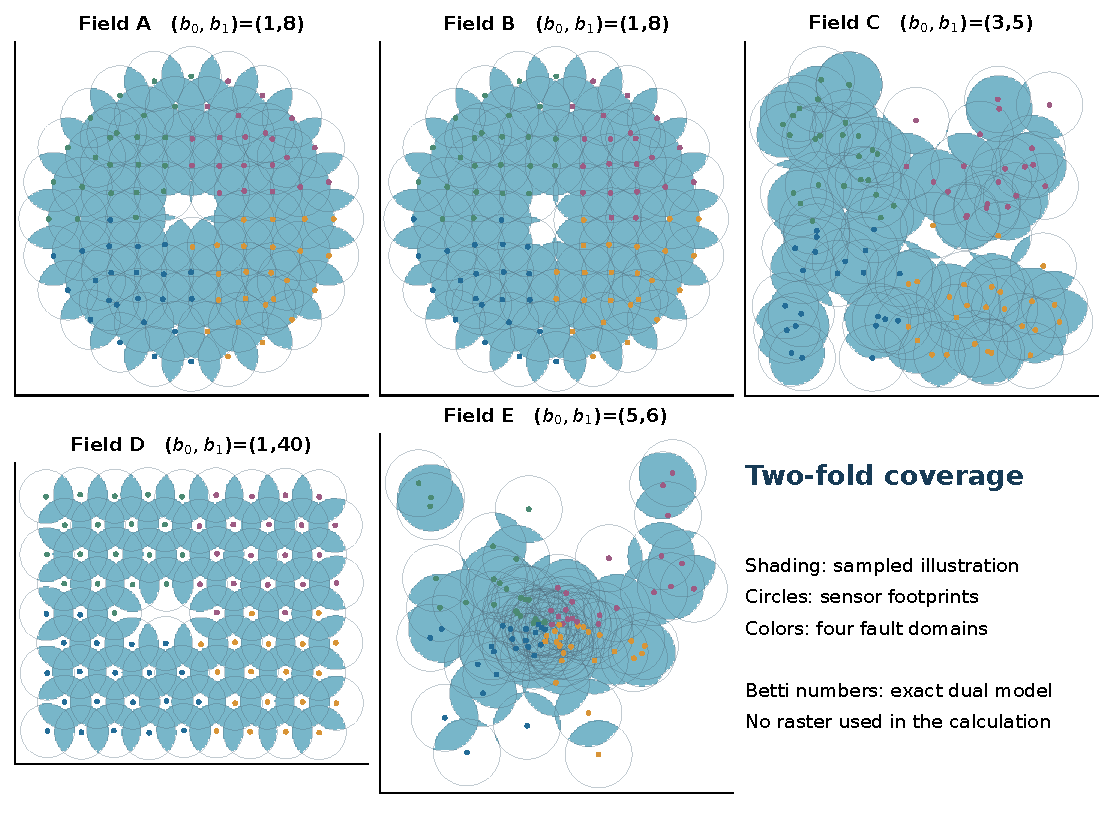
\includegraphics[width=\textwidth]{figures/five-fields.pdf}
\caption{The five fixed fields at two-fold coverage. Shading is a sampled illustration and can miss thin geometric features; it is not used to determine topology. The displayed Betti numbers come from the complete exact dual two-skeleton. Contact colors show the four deterministic domains in \cref{eq:domain-assignment}.}
\label{fig:fields}
\end{figure}
\FloatBarrier
\clearpage

\subsection{Complete dual counts}
\begin{longtable}{llrrrrrr}
\caption{Complete dual two-skeleton counts and Betti numbers. The domain model survives every loss of one of the four stated domains.}\label{tab:all-results}\\
\toprule Field & Rule & $V$ & $E$ & $T$ & $\rank\partial_2$ & $b_0$ & $b_1$ \\ \midrule\endfirsthead
\toprule Field & Rule & $V$ & $E$ & $T$ & $\rank\partial_2$ & $b_0$ & $b_1$ \\ \midrule\endhead
\bottomrule\endfoot
A & $k=1$ & 153 & 1821 & 8798 & 1668 & 1 & 1 \\
A & $k=2$ & 153 & 1037 & 2498 & 877 & 1 & 8 \\
A & $k=3$ & 153 & 533 & 615 & 342 & 4 & 42 \\
A & Domains & 45 & 100 & 84 & 59 & 4 & 0 \\
A & Budget & 153 & 854 & 1741 & 682 & 1 & 20 \\
\addlinespace
B & $k=1$ & 150 & 1753 & 8223 & 1603 & 1 & 1 \\
B & $k=2$ & 150 & 990 & 2263 & 833 & 1 & 8 \\
B & $k=3$ & 150 & 522 & 585 & 332 & 4 & 44 \\
B & Domains & 46 & 109 & 111 & 67 & 4 & 0 \\
B & Budget & 150 & 837 & 1710 & 667 & 1 & 21 \\
\addlinespace
C & $k=1$ & 107 & 987 & 3869 & 878 & 1 & 3 \\
C & $k=2$ & 107 & 678 & 1822 & 569 & 3 & 5 \\
C & $k=3$ & 105 & 456 & 842 & 343 & 4 & 12 \\
C & Domains & 38 & 126 & 209 & 89 & 1 & 0 \\
C & Budget & 107 & 589 & 1483 & 475 & 3 & 10 \\
\addlinespace
D & $k=1$ & 118 & 563 & 848 & 445 & 1 & 1 \\
D & $k=2$ & 118 & 157 & 0 & 0 & 1 & 40 \\
D & $k=3$ & 118 & 0 & 0 & 0 & 118 & 0 \\
D & Domains & 27 & 23 & 0 & 0 & 4 & 0 \\
D & Budget & 118 & 110 & 0 & 0 & 22 & 14 \\
\addlinespace
E & $k=1$ & 130 & 4617 & 107292 & 4488 & 2 & 1 \\
E & $k=2$ & 130 & 4214 & 94985 & 4083 & 5 & 6 \\
E & $k=3$ & 128 & 3910 & 85522 & 3795 & 16 & 3 \\
E & Domains & 104 & 3507 & 77706 & 3404 & 1 & 0 \\
E & Budget & 128 & 4120 & 90824 & 3994 & 6 & 4 \\
\addlinespace
\end{longtable}

All $25$ model computations use the same maximal nerve faces within their respective field. Only the winning test changes. The ring fields have identical two-fold Betti pairs $(1,8)$ but different higher-order and weighted results. The random field gives $(3,5)$ at two-fold coverage, illustrating that its topology cannot be established by a coarse raster comparison alone. Field~D has $118$ isolated three-fold components and no dual three-fold edges, whereas its two-fold graph has $157$ edges and no triangles, giving $40$ independent graph cycles.

The structured rules change the region in ways that a single overlap threshold does not capture. In Field~E, two-fold coverage gives $(5,6)$; survival of a complete domain loss gives $(1,0)$; the chosen weighted budget gives $(6,4)$. The domain-surviving region is a subset of the two-fold region, but removing parts of a region can delete whole components as well as remove or create holes. There is no monotonicity law for either Betti number separately under set inclusion.

\begin{figure}[!htbp]
\centering
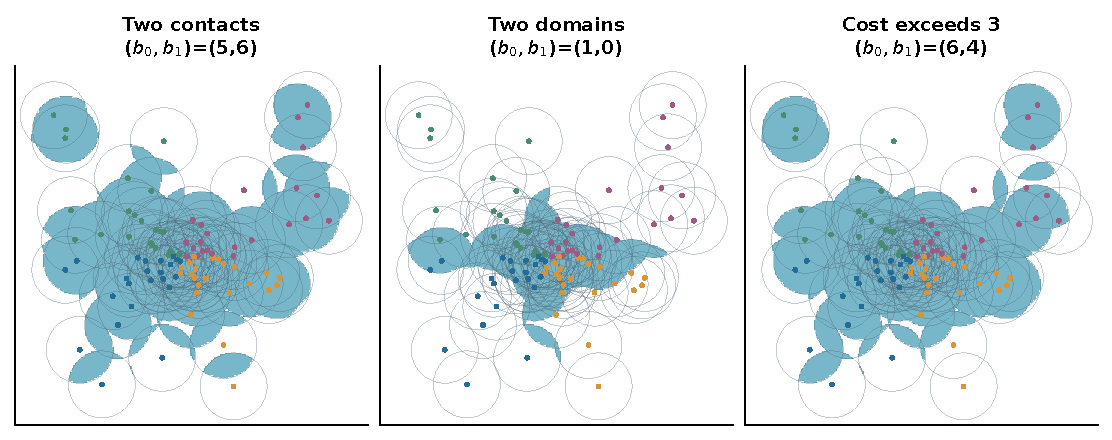
\includegraphics[width=\textwidth]{figures/structured-field-E.pdf}
\caption{Field~E under three distinct failure rules. Geometric shading is illustrative; exact counts are in \cref{tab:all-results}. Domain redundancy requires contacts from different groups, whereas the budget rule evaluates their stated deletion costs. None of these panels certifies coverage of an unstated external target.}
\label{fig:structured}
\end{figure}

\subsection{Completion and correction of the dense example}
The equal-radius nerve of Field~E has $95$ vertices, $1810$ edges and $24\,956$ triangles. An independent recount of the two-fold coalition shadow gives
\[
\abs{\Delta_2^{(0)}}=1810,\qquad
\abs{\Delta_2^{(1)}}=836\,991.
\]
Thus the number previously described as its vertex count is an edge count. This revision corrects the abstract, discussion and size comparison rather than carrying that description forward.

There are $130$ maximal nerve faces in the exact facet list. All $130$ win for two-fold coverage. In the dual complex the graph has $4214$ edges and five components, so its cycle-space dimension is
\[
4214-130+5=4089.
\]
The full list of $94\,985$ triangle columns has rank $4083$. It follows that
\[
b_1=4089-4083=6.
\]
The duality theorem transfers this finite calculation to the two-fold covered region. The calculation completes this one previously unfinished case. It is not a claim to resolve an unrelated open conjecture.

\begin{figure}[!htbp]
\centering
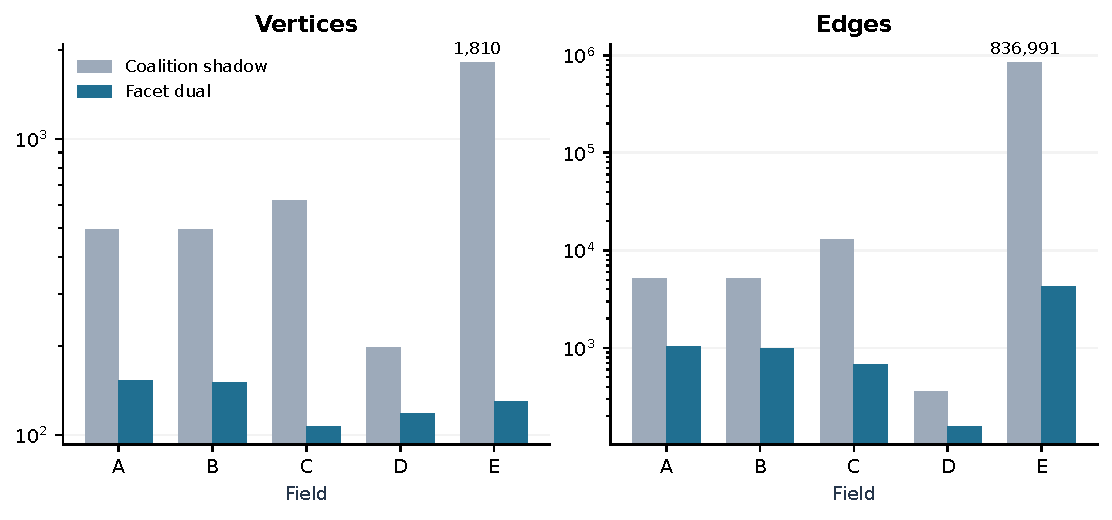
\includegraphics[width=\textwidth]{figures/compression.pdf}
\caption{Exact counts in the coalition-shadow and facet-dual representations for two-fold coverage. The vertical axes are logarithmic. The dual need not be smaller on every input, and these empirical reductions are not a universal linear-size theorem. The dense-field shadow has $1810$ vertices and $836\,991$ edges.}
\label{fig:compression}
\end{figure}
\FloatBarrier

\subsection{Independent checks and their scope}
The geometry audit compares every disk pair and triple with the facet face oracle: $125\,580$ tests in each ring field, $142\,880$ in each of Fields~C and~E, and $82\,160$ in Field~D, totaling $619\,080$ comparisons. There is no exact pair or triple tangency in these fixed fields. The audit additionally checks each returned facet using the equal-radius Helly criterion and checks that adjoining any absent contact destroys the face property. Field~E's ordinary pair and triple counts independently reproduce $1810$ and $24\,956$.

The two-fold boundary rank is recomputed with a separate set-column elimination that uses the smallest available pivot. The main routine uses integer bit columns with the largest available pivot. Both orders give ranks $877,833,569,0,4083$ for Fields~A--E. This is an independent arithmetic implementation of the rank check, not an independent proof-assistant formalization.

The control suite contains ten tests. Its exhaustive small geometric controls compare all nonempty subsets in $50$ seven-contact equal-radius fields with a different minimum-enclosing-circle oracle. Its combinatorial controls compare the dual and minimal-coalition models on $150$ random small nerves under four types of monotone rule, giving $600$ comparisons of $(b_0,b_1)$. Additional controls address exact tangency, a one-unit binary64 separation beyond tangency, unequal and coincident disks, zero radii, very small and very large power-of-two scales, radical signs, budget validation, correlated-domain failure and the continuous triangle certificate.

The geometric and combinatorial control tests are evidence about the implementation. The all-input assertions are established by the mathematical proofs, not by extrapolating the controls. In particular, matching all pair and triple tests would not by itself establish completeness of an arbitrary facet enumeration; \cref{thm:witness} supplies that missing logical guarantee.

\subsection{Reproducibility and limitations}
The repository contains the CSV inputs, radii, exact facet masks, all $25$ model counts, the separate geometric and rank audit, the corrected shadow edge recount and the figure generator. The main geometry and homology computations use Python's standard library; the figure generator additionally uses NumPy and Matplotlib. Figures are generated from the saved results and input coordinates. Rasterization occurs only in the illustrations.

The experiment does not compare performance against every existing multicover implementation, determine a practical optimal failure model or establish superiority over the bifiltration methods of~\cite{corbet,alonso}. Its purpose is a reproducible evaluation of the stated construction and a finite completion of the dense v2 example. Runtime observations depend on implementation and machine and are not used as asymptotic claims.

The current package does not provide a Lean formalization. Its exact computations concern $H_0$ and $H_1$ over $\FF$; they do not assert integral homology, all higher Betti numbers or clinical reliability. The target certificate is proved for closed planar triangles with the stated metric. A curved-surface implementation requires certified metric error bounds or another geometric certificate, as emphasized in the companion archive~\cite{ecog}.
\FloatBarrier

\appendix
\section{Order maps and the comparison homotopies}
\label{app:posets}
We spell out the finite order argument used in \cref{thm:duality}. For a poset $P$, its order complex has vertices $p\in P$ and simplices the nonempty chains. An order-preserving map sends chains to chains, possibly with repetitions; deleting repetitions gives a simplicial map. An order-reversing map does the same after reversing the order of the image chain. The order complexes of a poset and its opposite are therefore the same abstract complex.

\begin{lemma}[Order comparison homotopy]\label{lem:order-homotopy}
If $a,b:P\to Q$ are order-preserving maps of finite posets with $a(p)\le b(p)$ for all $p$, their induced maps on realizations are homotopic.
\end{lemma}
\begin{proof}
The map $H:P\times\{0<1\}\to Q$ defined by $H(p,0)=a(p)$ and $H(p,1)=b(p)$ is order preserving. The only mixed comparison needing verification is $(p,0)\le(p',1)$, which implies $p\le p'$ and hence $a(p)\le a(p')\le b(p')$. The order complex of this product triangulates each prism over a chain of $P$: a chain $p_0<\cdots<p_s$ is crossed with an interval and split at each possible transition from level zero to level one. These prism triangulations agree on shared faces. Realizing $H$ gives a continuous homotopy from the realization of $a$ to that of $b$.
\end{proof}

The maps $g f$ and $f g$ of \cref{eq:f-map,eq:g-map} are order preserving and lie above the identity. Applying \cref{lem:order-homotopy} gives both homotopies required there. This avoids choosing a maximal face for each simplex, which would obscure naturality when the failure rule changes.

An alternative intermediate model is the order complex of the winning-face poset $\cP_{\F}$. Define
\[
u:Q_\Gamma\longrightarrow\cP_{\F},\qquad u(A)=\bigcup_{\sigma\in A}\sigma,
\]
and
\[
t:\cP_{\F}\longrightarrow Q_\Gamma,\qquad
t(\sigma)=\{\tau\in\cP_{\F}:\tau\subseteq\sigma\}.
\]
These are order preserving, $u t$ is the identity, and $A\subseteq t u(A)$. Thus $\Gamma_{\F}$ is also homotopy equivalent to the winning-face order complex. For the cardinality rule, this is the subcomplex of the barycentric nerve subdivision on faces of size at least $k$, connecting the present formulation directly to the classical multicover nerve~\cite{sheehy}. The map $u$ commutes with inclusions of winning-face sets at fixed $N$.

\section{A chain comparison for the disk covers}
\label{app:nerve}
This appendix explains the natural homology statement in the semialgebraic disk setting without treating an arbitrary closed cover as an open good cover. A finite family of compact semialgebraic sets admits a common finite compatible triangulation~\cite{realalgebraic,bauer}. Apply this to the finitely many disk intersections appearing in the secondary covers under consideration. Each such set is represented by a subcomplex of a common finite complex $L$. Every nonempty finite intersection remains contractible because it is convex before triangulation.

Index one cover by a finite set $I$, write $L_i$ for its subcomplexes and $L_A=\bigcap_{i\in A}L_i$. Over a field, form the double-chain groups
\begin{equation}\label{eq:double-chain}
E_{p,q}=\bigoplus_{\substack{A\subseteq I\\|A|=p+1}}C_q(L_A),\qquad p,q\ge0,
\end{equation}
omitting empty intersections. The vertical boundary is the simplicial boundary of $L_A$. The horizontal boundary is the alternating sum of inclusions obtained by dropping one index of $A$. The standard total sign convention makes the total differential square to zero; over $\FF$ the signs disappear.

Augment horizontally to the chain complex of the union. For a fixed simplex $s$ of the union, let $I_s=\{i:s\in L_i\}$. This set is nonempty. Its copies in the augmented row of \cref{eq:double-chain} form precisely the augmented chain complex of the full simplex on $I_s$. That complex is exact: fixing one index in $I_s$ and adjoining it gives a contracting homotopy. Splitting the row over the simplices $s$ proves horizontal exactness. Thus the total chain complex computes the homology of the union.

In the other direction, take vertical homology first. Each nonempty $L_A$ is contractible, so it has one-dimensional ordinary $H_0$ and zero higher homology. Sending every vertex of a connected $L_A$ to $1$ identifies its $H_0$ with the coefficient field compatibly with inclusion. The remaining horizontal complex is exactly the simplicial chain complex of the nerve. The two filtrations of the finite double complex therefore identify nerve homology with union homology. This can be expressed as the two elementary finite spectral-sequence comparisons, or by successive elimination of the exact augmented rows and the positive-degree acyclic columns.

If a cover subfamily is included in a larger cover, the same triangulation can be used for both, and inclusion of summands in \cref{eq:double-chain} commutes with both augmentations. Hence the resulting homology isomorphisms are natural. No human choice of one witness point per nerve simplex enters the induced homology comparison. The general closed-convex homotopy theorem used in \cref{thm:duality} is the standard theorem cited in~\cite{bauer}; this appendix supplies a detailed homological explanation for the disks actually computed.

\section{Boundary arithmetic and exact input semantics}
\label{app:arithmetic}
\subsection{Binary columns over \texorpdfstring{$\FF$}{F2}}
Number the dual edges from zero to $E-1$. A triangle with edge indices $a,b,c$ has boundary column
\[
z=2^a\mathbin{\oplus}2^b\mathbin{\oplus}2^c,
\]
where $\oplus$ is bitwise exclusive-or. This is simply an encoding of a vector in $\FF^E$; it is not integer linear algebra. Each edge has two vertex endpoints, so applying the edge boundary to a triangle boundary counts every vertex twice. Therefore $\partial_1\partial_2=0$.

To compute the rank, maintain at most one pivot column for each leading nonzero row. A new column is repeatedly added to the stored column with the same leading row until it becomes zero or acquires a previously unused leading row. In the latter case store it. Every reduction step preserves the span of columns seen so far. Stored columns have distinct leading rows and are linearly independent. Each processed column is in their span, so the number stored is exactly the boundary rank. Termination follows because the leading nonzero row strictly decreases in the main implementation.

The independent audit represents columns by sets and instead uses the smallest nonzero row. That leading row strictly increases. Its correctness follows from the same span invariant, but its representation and pivot trajectory differ. Agreement is useful for detecting implementation errors, while the invariant supplies the proof of either algorithm for every finite input.

\subsection{Rational comparisons and equality}
A finite binary64 number is a rational of the form $m2^e$. The input conversion preserves that value as a Python \texttt{Fraction}. Products, sums and divisions in \cref{eq:circle-parameters,eq:quadratic-membership,eq:mec} therefore have exact integer numerators and denominators. The only radicals are eliminated by the signed comparisons of \cref{lem:sign}. Unconditional squaring would be wrong when the compared sides have uncontrolled signs; the sign cases are part of the algorithm.

The geometry API explicitly converts supplied numerical values to binary64 before making their rational representations. Passing a rational with a non-dyadic denominator to that API does not request symbolic preservation of the original rational; it requests exact treatment of its binary64 conversion. The abstract rational algorithm of \cref{thm:algorithm} can instead be implemented with rational inputs directly. The released computations consistently use the former convention and record the input hashes.

No geometric epsilon is used to merge circles, enlarge radii or decide tangency. Equal centers are tested as exact rational pairs. Coincident disks retain distinct labels because a failure model can distinguish the two contacts even when their geometry is identical. Equality in a closed-disk test is accepted. The companion archive's open-disk routines~\cite{ecog} use strict inequalities, so they must not be interchanged without specifying the convention.

\section{Counterexamples to stronger interpretations}
\label{app:counterexamples}
\begin{example}[Hole-free does not imply target coverage]
Let $D_1$ be the unit disk at the origin and let the target be the unit disk centered at $(10,0)$. The ordinary covered region is contractible and has $b_1=0$, but its intersection with the target is empty. No theorem using only the absolute Betti numbers of the covered region can certify containment of every possible externally supplied target.
\end{example}

\begin{example}[Pairwise overlap does not determine a triangle]
Three disks centered at the vertices of an equilateral triangle of side $d$ overlap pairwise when $r\ge d/2$, but share a common point only when $r\ge d/\sqrt3$. For $d/2<r<d/\sqrt3$, their nerve contains a cycle without a filled triangle. Replacing the nerve by the flag complex of pairwise overlaps changes $H_1$. The same issue appears again in the facet-intersection model, as noted after \cref{prop:two-skeleton}.
\end{example}

\begin{example}[Geometric uncertainty can hide temporary homology]
Even when an inner region and an outer region are both disks, an intermediate subset containing the inner disk and contained in the outer disk can be an annulus attached to that disk, or a disk with a separate small component. Thus knowledge of endpoint Betti numbers alone does not determine all intermediate Betti numbers. The rank lower bound after \cref{thm:stability} is the conclusion that follows from the factorization; a stronger exactness assertion would require additional hypotheses.
\end{example}

\section{Revision record and reproducible commands}
The present v3 changes the title to reflect the failure-family extension, adds Sanjeevan Singha Roy as the third author, preserves the two original authors, corrects the dense-field vertex/edge description, replaces the unfinished dense calculation by a complete dual computation and separates target containment from absolute homology. It supplies explicit proofs and arithmetic conventions rather than appending an unrelated paper.

From the repository root, with a standard Python installation, the scientific checks are:
\begin{verbatim}
python -m unittest discover -s code -v
python code/run_fields.py
python code/verify_fields.py
python code/audit_shadow_edges.py
\end{verbatim}
Only the figure generator requires NumPy and Matplotlib:
\begin{verbatim}
python code/make_figures.py
\end{verbatim}
The figures and generated table are already included in the TeX package. For a first build with an ordinary LaTeX installation, run \texttt{pdflatex main.tex} three times in the \texttt{paper} directory so that the contents and cross-references stabilize. Overleaf normally handles these passes automatically. No external article PDF is embedded in the manuscript. The bibliography cites the specific earlier works relevant to its definitions, methods or context.

The public source is the \href{https://github.com/creelie/nerve-coverage-v3}{nerve-coverage-v3 repository}. The DOI \href{https://doi.org/10.5281/zenodo.23731783}{10.5281/zenodo.23731783} identifies the companion ECoG archive cited in this paper; it is not presented as the DOI of this v3.

\paragraph{Preparation tools.}
OpenAI Codex assisted with the revision's mathematical exposition, code, numerical audits and figure preparation. The package supplies the arguments, executable checks and their stated scope for inspection. This assistance is distinct from proof-assistant formalization. The human authors remain responsible for reviewing the final work and for submission declarations.

\begin{thebibliography}{99}
\bibitem{original}
D.~Bhattacharjee and U.~Bhattacharya,
\emph{Iterated Nerve Complexes for $k$-Fold Sensor Coverage},
Preprints.org, version 2, 2026.
\href{https://doi.org/10.20944/preprints202606.1351.v2}{doi:10.20944/preprints202606.1351.v2}.

\bibitem{ecog}
A.~Bose, D.~Bhattacharjee and U.~Bhattacharya,
\emph{Certified Redundant ECoG Coverage: Exact Geometry, Continuous Mesh Certificates and Reproducible Audits},
research and software archive, version 1.6.0, Zenodo, 2026.
\href{https://doi.org/10.5281/zenodo.23731783}{doi:10.5281/zenodo.23731783}.

\bibitem{sheehy}
D.~R.~Sheehy,
\emph{A multicover nerve for geometric inference},
Proceedings of the 24th Canadian Conference on Computational Geometry, Charlottetown, 2012.
\url{https://mathtube.org/sites/default/files/lecture-notes/e-proceedings.pdf}.

\bibitem{corbet}
R.~Corbet, M.~Kerber, M.~Lesnick and G.~Osang,
\emph{Computing the multicover bifiltration},
Discrete Comput. Geom. \textbf{70} (2023), 376--405.
\href{https://doi.org/10.1007/s00454-022-00476-8}{doi:10.1007/s00454-022-00476-8}.

\bibitem{alonso}
\'{A}.~J.~Alonso,
\emph{A sparse multicover bifiltration of linear size},
Discrete Comput. Geom., published online August 4, 2026.
\href{https://doi.org/10.1007/s00454-026-00865-3}{doi:10.1007/s00454-026-00865-3}.

\bibitem{dowker}
C.~H.~Dowker,
\emph{Homology groups of relations},
Ann. of Math. (2) \textbf{56} (1952), 84--95.
\href{https://doi.org/10.2307/1969768}{doi:10.2307/1969768}.

\bibitem{chowdhury}
S.~Chowdhury and F.~M\'emoli,
\emph{A functorial Dowker theorem and persistent homology of asymmetric networks},
J. Appl. Comput. Topol. \textbf{2} (2018), 115--175.
\href{https://doi.org/10.1007/s41468-018-0020-6}{doi:10.1007/s41468-018-0020-6}.

\bibitem{bauer}
U.~Bauer, M.~Kerber, F.~Roll and A.~Rolle,
\emph{A unified view on the functorial nerve theorem and its variations},
Expo. Math. \textbf{41} (2023), no.~4, article 125503.
\href{https://doi.org/10.1016/j.exmath.2023.04.005}{doi:10.1016/j.exmath.2023.04.005}.

\bibitem{ghrist}
R.~Ghrist and A.~Muhammad,
\emph{Coverage and hole-detection in sensor networks via homology},
Proceedings of IPSN 2005, IEEE, 2005, 254--260.

\bibitem{desilva}
V.~de Silva and R.~Ghrist,
\emph{Coverage in sensor networks via persistent homology},
Algebr. Geom. Topol. \textbf{7} (2007), 339--358.
\href{https://doi.org/10.2140/agt.2007.7.339}{doi:10.2140/agt.2007.7.339}.

\bibitem{controlled}
V.~de Silva and R.~Ghrist,
\emph{Coordinate-free coverage in sensor networks with controlled boundaries via homology},
Int. J. Robot. Res. \textbf{25} (2006), 1205--1222.

\bibitem{realalgebraic}
J.~Bochnak, M.~Coste and M.-F.~Roy,
\emph{Real Algebraic Geometry},
Ergebnisse der Mathematik und ihrer Grenzgebiete (3), vol.~36, Springer, Berlin, 1998.
\href{https://doi.org/10.1007/978-3-662-03718-8}{doi:10.1007/978-3-662-03718-8}.

\bibitem{topoi}
D.~Bhattacharjee,
\emph{Neuromorphic Grothendieck topoi for grid-embedded circuit architectures},
SSRN, 2026.
\href{https://doi.org/10.2139/ssrn.6194939}{doi:10.2139/ssrn.6194939}.

\bibitem{suspension}
D.~Bhattacharjee,
\emph{Suspension of structures in two-dimensional topologies with or without the presence of $\mathcal X\ge1$ genus deformations for canonical $2^{2\eta}$ stabilizer points},
Research Square, version 1, 2022.
\href{https://doi.org/10.21203/rs.3.rs-1798323/v1}{doi:10.21203/rs.3.rs-1798323/v1}.

\bibitem{linkage}
S.~Singha Roy, D.~Bhattacharjee and R.~Sadhu,
\emph{Instability in the linkage of topological spaces due to background ghosts},
EPRA Int. J. Res. Dev. \textbf{8} (2023), no.~4, 276--279.
\href{https://doi.org/10.36713/epra13019}{doi:10.36713/epra13019}.
\end{thebibliography}

\end{document}
